\documentclass[10pt]{article}

\usepackage{atml}

\input{math_commands.tex}

\usepackage{hyperref}
\usepackage{url}
\usepackage{graphicx}
\usepackage{booktabs}
\usepackage{multirow}
\usepackage{xcolor}

\graphicspath{{figures/}}

\title{Reproducing SRSNet: a closer look at Selective Patching
and Adaptive Fusion}

\author{%
  \name Andrea Perugini \email peruga@usi.ch
  \AND
  \name Dominik Panzarella \email panzad@usi.ch
  \AND
  \name Susanna Ardig\`o \email ardigs@usi.ch
}

\def\groupid{---}
\def\projectid{SRSNet-Repro}


\begin{document}

\maketitle

\begin{abstract}
In this work, we reproduced the ETT-facing experiments of SRSNet using the released code and methods. Since the full
benchmark was too expensive on our available hardware and some released scripts were incomplete, we restricted the
reproduction to the four ETT datasets and four forecast horizons. SRSNet remains close to the strongest baselines,
particularly on MAE, but the numerical results differ from the paper and fail to display the clear
dominance reported by the authors. As a follow-up, we tested several controls for the SRS mechanism, replacing
learned selection with random or engineered alternatives, and we also introduced a context-dependent hypernetwork
in lieu of the fixed fusion weight. Our extensions remain within the observed seed-level variation, thereby
suggesting that, at least insofar as our reproduction scope is concerned, we cannot clearly isolate learned Selective
Patching as the main source of SRSNet's performance.
\end{abstract}

\section{Background and model}

\paragraph{Patching in time series forecasting.}
Long-term time series forecasting predicts the next $L$ values
given a lookback window of past observations $X \in \mathbb{R}^{N
\times T}$ with $N$ channels and $T$ timesteps. Recent work has
converged on a simple recipe inspired by Vision Transformers: cut
the lookback into short \emph{patches}, embed each patch into a
vector, run a backbone over the patch tokens, and read the
forecast from a small head. PatchTST \citep{nie2023patchtst},
Crossformer \citep{zhang2022crossformer} and PatchMLP
\citep{tang2025patchmlp} all share this template, channel-
independent strategy included. Patches make the input more
semantically rich than a single timestep, and reduce the sequence
length the backbone has to deal with.

\paragraph{The problem the paper raises.}
All these models cut the lookback into \emph{adjacent} patches
with fixed stride $s$. The slicing is the same for every input
and every dataset. \citet{wu2025srsnet} argue that this is
limiting on three fronts: a fixed grid can split distribution-
shift boundaries (changes of regime, anomalies, shifts) in the
middle of a patch; quasi-periodic signals produce consecutive
patches that are near-copies of each other; and the choice does
not adapt to the data. The paper's claim is that a more flexible
patching, picked from the input itself, should help.

\paragraph{The SRS module.}
The proposed module, called the \emph{Selective Representation
Space} (SRS), builds two views of the same window and blends
them. The first view is the conventional adjacent patching
already used by every other patch-based model. The second view,
the \emph{selective view}, is constructed in two steps.

\emph{Selective Patching} (SP) considers every possible sub-window of
length $p$ at stride $1$ (so $K = (n-1)\,s + 1$ candidates with
$T = 96$, $p = 24$ and $s = 24$, this gives $73$ candidates) and
scores each candidate with a small MLP, the \emph{Scorer$^s$}. Argmax
over the score axis then selects the top $n$ candidates.

\emph{Dynamic Reassembly} feeds the $n$ selected patches into a
second MLP, the \emph{Scorer$^r$}, which scores each one. Argsort then
turns these scores into an ordering: for example, scores
$[0.3, 0.9, 0.1]$ would place the second patch first.

Because both Argmax and Argsort are non-differentiable, the paper
uses a straight-through trick to propagate gradients back to the
two scorers: each selected (or reordered) patch is multiplied by
a tensor that is numerically equal to $1$ but carries the gradient
of the scorer's output. This is what allows the scorers to be
trained end-to-end with the rest of the model.

Both views, after their own linear patch-embedding, become two
tensors $E^c, E^s \in \mathbb{R}^{N \times n \times d}$. The
\emph{Adaptive Fusion} (AF) merges them with a learned weight
$\alpha \in [0, 1]^{n \times d}$:
\[
\tilde{E} \;=\; \alpha \odot E^c + (1 - \alpha) \odot E^s.
\]
In practice $\alpha$ is a free \texttt{nn.Parameter} of shape
$[n, d_\text{model}]$ wrapped in a sigmoid so the constraint
$\alpha \in [0, 1]$ is satisfied automatically. It is learned
during training but does not depend on the input at inference
time: the same $\alpha$ is applied to every forward pass once
training is done. The paper itself flags this in its future work section
as a place where a more adaptive mechanism could
help. A sinusoidal positional embedding is finally added on
top.

\paragraph{SRSNet.}
The released implementation uses RevIN \citep{kim2022revin}, the SRS module, and a FlattenHead.
Figure~\ref{fig:srs-pipeline} shows the full
pipeline reproduced from the paper.

\begin{figure}[t]
  \centering
  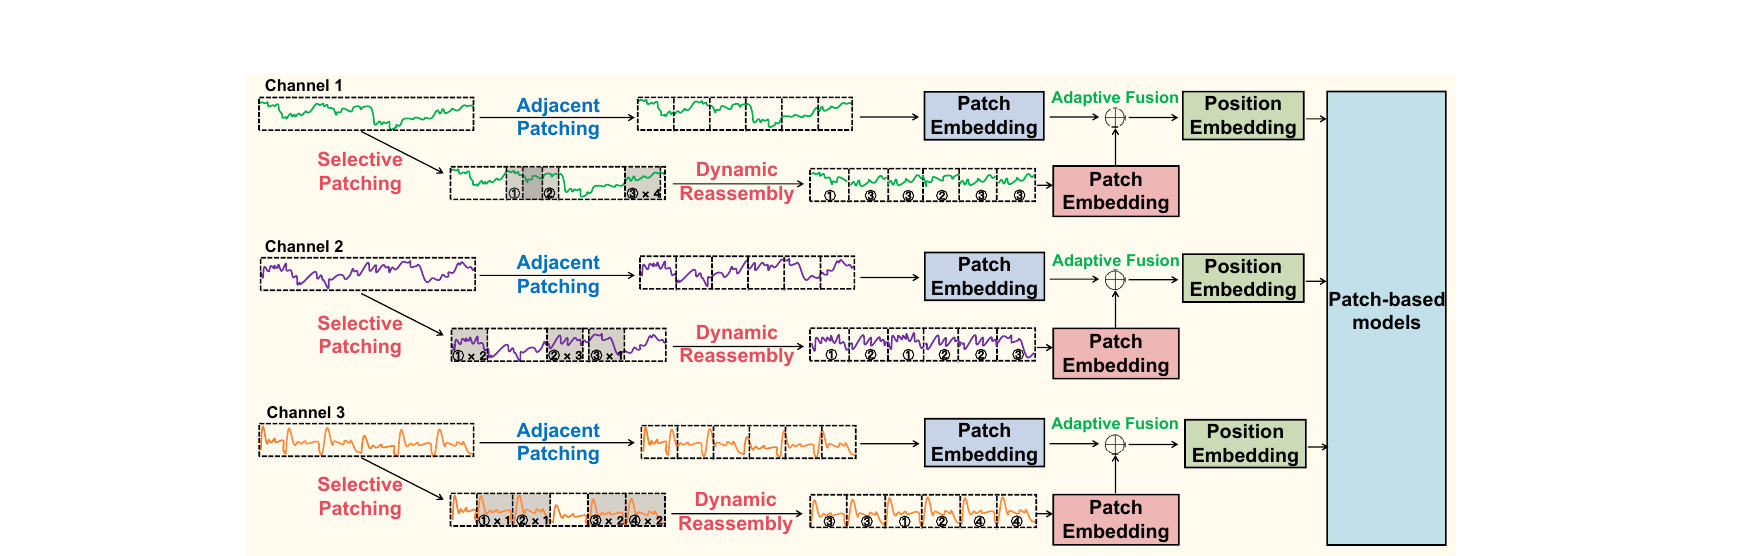
\includegraphics[width=0.95\linewidth]{fig2_pipeline}
  \caption{SRSNet pipeline (reproduction of
    \citealt[Fig.~2]{wu2025srsnet}). The adjacent and selective
    streams are linearly embedded, blended by the Adaptive Fusion
    through $\alpha$, summed with a sinusoidal positional
    embedding, and passed to the linear head.}
  \label{fig:srs-pipeline}
\end{figure}


This makes SRSNet a useful reproducibility target for two reasons. First, the paper
reports strong benchmark results against several forecasting models. Second, we can actually take apart and
test its claimed mechanism, i.e., if learned SP is central to the model, then randomising or removing altogether
the selector should hurt performance. Our report can therefore be divided into two parts: we first
reproduced the ETT-facing experiments across the headline comparison, the plug-in study, and ablation; we
then ran extensions targeting the learned selection, the fusion weight, and the forecasting head.

\section{What we wanted to test}
\label{sec:stuff-to-test}

The paper makes two claims that are relevant to our project: first,
that the SRS module improves over a simple MLP forecaster; second, 
that the individual SRS components (namely, Selective Patching, Dynamic Reassembly,
and Adaptive Fusion) are important, with their ablation study attributing the greatest impact to
Selective Patching. Thus, on top of reproducing these tests, we wanted to
test whether the learned selector itself was necessary as a complementary control \textbf{RandomSP}.
We kept the selective-patching structure, but replaced the learned top-k scoring
with random selection. Therefore, if learned patch selection is responsible for the
observed gain, using random choices should hurt consistently.
As a stricter version of this control, \textbf{RandomSPNoShuffle} additionally
disables the learned Scorer$^r$ (Dynamic Reassembly), so the random patches are
kept in the order in which they were sampled. This way, we also probe whether the
learned reordering carries any independent value beyond the selection itself.


After that destructive control, we also introduced two other constructive variants
in our extensions. Time-Aware Selective Patching (\textbf{TASP}) swaps the raw patch scoring
input with four simple time-series descriptors, so we explore whether patch selection can be made both more
interpretable and more efficient. In practice, the engineered features that we chose are dominant FFT magnitude,
lag-1 autocorrelation, variance, and trend slope. Next, Hypernet Adaptive Fusion (\textbf{HypernetAF}) instead does not target
the selector, but it replaces the static fusion parameter $\alpha$ with a small per-batch context-dependent two-layer network.
More explicitly, in vanilla SRSNet the adjacent-patch embedding $E^c$ and the selective/reassembled embedding $E^s$ are combined
using a learned tensor $\alpha \in [0,1]^{n \times d}$ (in practice a free \texttt{nn.Parameter} wrapped in a sigmoid of shape $[n, d_\text{model}]$ like in the standard AF explained above):
  \[
  \tilde{E} = \alpha \odot E^c + (1 - \alpha) \odot E^s.
  \]
This tensor is learned during training, but at inference the same fusion weights are used
for every input.
Conversely, in HypernetAF, after computing the
adjacent-view embedding $E^c$, we average it over the batch/channel axis and over patches
to obtain a context vector $c \in \mathbb{R}^d$. This context is passed through a small
two-layer network whose output is reshaped and wrapped in the same sigmoid as vanilla AF:
  \[
  h = \mathrm{ReLU}(W_1 c + b_1), \qquad
  \alpha_{\mathrm{dyn}} = \mathrm{sigmoid}\!\bigl(\mathrm{reshape}(W_2 h + b_2)\bigr),
  \]
with $\alpha_{\mathrm{dyn}} \in [0,1]^{n \times d}$. The output bias $b_2$ is initialised to
$3.5$, so at step~$0$ every component of $\alpha_{\mathrm{dyn}}$ is $\sigma(3.5) \approx 0.97$,
matching the vanilla initialisation used by the authors in the ETTh1 scripts. This extension was further motivated by
the fact that Adaptive Fusion emerged as the most influential component in our reproduced ablation.
If fusion is indeed important, we might improve robustness by letting the fusion weight depend on the
batch context.

Lastly, to check whether the simple linear forecasting head is a bottleneck, we tested the inclusion
of a small Transformer encoder following the SRS embedding. In practice, the encoder is a
standard \texttt{nn.TransformerEncoder} with two layers, four attention heads, and a feedforward
dimension equal to $4 d_{\mathrm{model}}$, inserted between the SRS module and the FlattenHead.
To probe whether the encoder interacts with the selection or fusion side, we re-ran three variants
in combination with it: vanilla SRSNet, TASP, and HypernetAF.


\section{Reproducibility}
\label{sec:results-repro}

We ran the experiments in the paper through the official TFB pipeline
\citep{qiu2024tfb} with paper-faithful overrides
(\texttt{batch\_size=64}, \texttt{train\_drop\_last=false},
\texttt{num\_workers=0}). All runs were on a single RTX 4090
($24$ GB) on Hivenet. A part of the runs was also double-tested
locally on the same GPU with comparable outcomes (results not reported
here). 

The paper covers eight benchmark datasets (the four ETT, plus
Weather, Solar, Traffic, Electricity). Running the full grid on our
hardware would have proven very time-consuming, as a single SRSNet run on Traffic or
Electricity at horizon $720$ takes several wall-clock hours with a batch size of $64$.
Thus, we narrowed down our scope to the four ETT
datasets (ETTh1, ETTh2, ETTm1, and ETTm2) and the four standard horizons (96, 192, 336, 720).
Within this scope, the headline comparison
covered SRSNet and the main released baselines used in the paper:
PatchTST, DLinear, iTransformer, TimesNet, TimeMixer, and PatchMLP.
Coverage was still not uniform: the released ETTh1
scripts for DLinear, iTransformer, TimesNet, and TimeMixer are
empty, while PatchMLP scripts are absent for ETTh2 and
ETTm1. We therefore report missing cells explicitly rather than
filling them with non-paper-faithful runs.
\subsection{Headline comparison (paper Tab.~2)}

Table~\ref{tab:tab2} averages MSE and MAE over the four horizons
for each (model, dataset) pair. PatchTST is generally strongest on
MSE, while SRSNet is especially competitive on MAE. Nonetheless, the grid does
not reproduce a clear dominance by SRSNet.
The non-Transformers baselines are not dominated, as DLinear and TimeMixer
remain competitive on several ETT columns, which is in line with prior work showing that simple
linear models can be strong time-series baselines \citep{zeng2023dlinear}.

The signed gap between our SRSNet numbers and the paper's averages
$|\Delta| \approx 18\%$ in absolute value. The signed differences are
structured by dataset, with ETTh1 and ETTm1 achieving worse results than the paper,
while ETTh2 and ETTm2 often appear better. We could not identify a single cause for the
discrepancies, and possible contributing factors might include hardware, nondeterministic kernels,
and small environment differences.


\begin{table}[t]
  \caption{Multivariate forecasting results, averages over horizons
    $F \in \{96, 192, 336, 720\}$. \textcolor{red}{\textbf{Red}}:
    best. \textcolor{blue}{\underline{Blue}}: 2nd best. Dash:
    missing or empty released script. Full per-cell
    numbers in Appendix~\ref{app:tab2-mae}.}
  \label{tab:tab2}
  \begin{center}
  \footnotesize
  \setlength{\tabcolsep}{4pt}
  \begin{tabular}{l|cc|cc|cc|cc}
    \toprule
    Datasets & \multicolumn{2}{c|}{ETTh1} & \multicolumn{2}{c|}{ETTh2}
             & \multicolumn{2}{c|}{ETTm1} & \multicolumn{2}{c}{ETTm2} \\
    Metrics  & MSE & MAE & MSE & MAE & MSE & MAE & MSE & MAE \\
    \midrule
    PatchTST     & \textcolor{red}{\textbf{0.521}} & \textcolor{blue}{\underline{0.517}} & \textcolor{red}{\textbf{0.306}} & \textcolor{red}{\textbf{0.378}} & \textcolor{red}{\textbf{0.400}} & 0.430 & \textcolor{red}{\textbf{0.206}} & \textcolor{blue}{\underline{0.300}} \\
    DLinear      & -- & -- & \textcolor{blue}{\underline{0.313}} & 0.389 & 0.406 & \textcolor{red}{\textbf{0.420}} & 0.208 & 0.303 \\
    iTransformer & -- & -- & 0.320 & 0.384 & 0.420 & 0.438 & 0.223 & 0.314 \\
    TimesNet     & -- & -- & 0.341 & 0.395 & 0.527 & 0.494 & 0.238 & 0.319 \\
    TimeMixer    & -- & -- & 0.319 & 0.387 & 0.410 & 0.426 & 0.211 & 0.305 \\
    PatchMLP     & 0.551 & 0.533 & -- & -- & -- & -- & 0.220 & 0.311 \\
    \midrule
    \textbf{SRSNet} & \textcolor{blue}{\underline{0.528}} & \textcolor{red}{\textbf{0.516}} & 0.314 & \textcolor{blue}{\underline{0.379}} & \textcolor{blue}{\underline{0.404}} & \textcolor{blue}{\underline{0.426}} & \textcolor{blue}{\underline{0.206}} & \textcolor{red}{\textbf{0.300}} \\
    \bottomrule
  \end{tabular}
  \end{center}
\end{table}

\subsection{Plug-in study (paper Tab.~3)}

In the plug-in comparison, we investigate the contribution of SRS on
top of an MLP backbone. While the paper reports improvements in MSE and MAE
in a range of $4$--$9\%$, the per-dataset average results of our reproduction
reported in Table~\ref{tab:tab3} show that adding SRS gives mixed, mostly small
changes. SRS has lower measured MSE in 7 of 16 cells, but the majority of the differences
are close to zero. We also did not find a clear long-horizon benefit; for example, at
horizon 720, SRS outperforms the baseline in only one dataset (ETTm1), and that margin is
negligible ($-0.03\%$). The ETTm1 dataset is also the only one showing lower measured MSE at all
time horizons.

\begin{table}[t]
  \caption{Plug-in study: MLP base (SRSNet w/o SRS) vs.\ SRSNet
    Full. Per-dataset averages across the four horizons. Improve\%
    is the relative MSE drop (positive means $+$SRS is better).}
  \label{tab:tab3}
  \begin{center}
  \footnotesize
  \setlength{\tabcolsep}{4pt}
  \begin{tabular}{l|cc|cc|cc|cc}
    \toprule
    Datasets & \multicolumn{2}{c|}{ETTh1} & \multicolumn{2}{c|}{ETTh2}
             & \multicolumn{2}{c|}{ETTm1} & \multicolumn{2}{c}{ETTm2} \\
    Metrics  & MSE & MAE & MSE & MAE & MSE & MAE & MSE & MAE \\
    \midrule
    MLP base ($=$ SRSNet w/o SRS) & 0.528 & 0.514 & 0.306 & 0.375 & 0.409 & 0.426 & 0.203 & 0.296 \\
    $+$SRS ($=$ SRSNet Full)      & 0.527 & 0.515 & 0.312 & 0.379 & 0.402 & 0.425 & 0.207 & 0.299 \\
    \midrule
    Improve (MSE)                 & \multicolumn{2}{c|}{$+0.03\%$} & \multicolumn{2}{c|}{$-1.82\%$}
                                  & \multicolumn{2}{c|}{$+1.91\%$} & \multicolumn{2}{c}{$-1.82\%$} \\
    \bottomrule
  \end{tabular}
  \end{center}
\end{table}

\subsection{Ablation (paper Tab.~4)}

The component ranking in our ablation differs notably from the paper. The authors flagged Selective
Patching as the largest individual contributor, while we identify that only removing Adaptive Fusion
results in a clear increase of average MSE as per Table~\ref{tab:tab4}. Concretely, removing AF
costs about $+3.4\%$ average MSE across the 16 ETT cells, whereas removing SRS as a whole, the
Selective Patching alone, or the Dynamic Reassembly alone all stay within roughly $0.1\%$ of the
full model. Therefore, within our reproduction scope, AF appears to be the component carrying most of the measurable contribution of SRS and this is the strongest reproducible finding of our study, while SP and DR are not separable from a baseline that does not use them


\begin{table}[t]
  \caption{Ablation of key components in SRS, averages over
    horizons. \textcolor{red}{\textbf{Red}}: best.
    \textcolor{blue}{\underline{Blue}}: 2nd best. Per-cell numbers
    in Appendix~\ref{app:tab4-mae}.}
  \label{tab:tab4}
  \begin{center}
  \footnotesize
  \setlength{\tabcolsep}{4pt}
  \begin{tabular}{l|cc|cc|cc|cc}
    \toprule
    Datasets & \multicolumn{2}{c|}{ETTh1} & \multicolumn{2}{c|}{ETTh2}
             & \multicolumn{2}{c|}{ETTm1} & \multicolumn{2}{c}{ETTm2} \\
    Metrics  & MSE & MAE & MSE & MAE & MSE & MAE & MSE & MAE \\
    \midrule
    w/o SRS                & \textcolor{blue}{\underline{0.528}} & \textcolor{red}{\textbf{0.514}} & \textcolor{red}{\textbf{0.306}} & \textcolor{red}{\textbf{0.375}} & 0.409 & \textcolor{blue}{\underline{0.426}} & \textcolor{red}{\textbf{0.203}} & \textcolor{red}{\textbf{0.296}} \\
    w/o Selective Patching & 0.528 & \textcolor{blue}{\underline{0.514}} & \textcolor{blue}{\underline{0.306}} & \textcolor{blue}{\underline{0.375}} & 0.408 & \textcolor{red}{\textbf{0.425}} & \textcolor{blue}{\underline{0.204}} & \textcolor{blue}{\underline{0.296}} \\
    w/o Dynamic Reassembly & 0.529 & 0.518 & 0.309 & 0.378 & \textcolor{blue}{\underline{0.403}} & \textcolor{blue}{\underline{0.426}} & 0.205 & 0.299 \\
    w/o Adaptive Fusion    & 0.551 & 0.538 & 0.323 & 0.390 & 0.406 & 0.430 & 0.216 & 0.310 \\
    \midrule
    \textbf{SRSNet (Full)} & \textcolor{red}{\textbf{0.526}} & 0.515 & 0.313 & 0.379 & \textcolor{red}{\textbf{0.403}} & 0.426 & 0.205 & 0.299 \\
    \bottomrule
  \end{tabular}
  \end{center}
\end{table}

\section{Extension results}
\label{sec:results-ext}

We trained the four single-axis variants of
Section~\ref{sec:stuff-to-test} (RandomSP, RandomSPNoShuffle, TASP,
HypernetAF) and a SRSNet baseline on the full ETT grid ($4$
datasets $\times$ $4$ horizons $\times$ $5$ seeds). Each variant
produces $80$ paired observations against SRSNet.
Before this full-grid run, we also ran a small $9$-variant pilot with
selection--fusion combinations on ETTh1 and ETTm2 at horizons $96$
and $720$; since the combinations did not show a clearer pattern, we
kept them in Appendix~\ref{app:small-grid-combos} and focused the
main text on single-axis variants.

Table~\ref{tab:variant-cells} reports the per-dataset averages over
horizons. The five variants land within $0.001$--$0.003$ MSE of each
other on every column: read at this resolution, replacing the
learned scorer with random selection (RandomSP / RandomSPNoShuffle),
using engineered features instead of raw patches (TASP), or making
$\alpha$ a function of the batch context (HypernetAF) produces no
visible difference from the baseline.

Aggregating the $80$ paired deltas (Table~\ref{tab:variant-stats})
gives the same picture in summary form. The mean $\Delta$MSE is at
most $0.35\%$ in magnitude for every variant; the seed-level
standard deviation is $\sim 2\%$, an order of magnitude larger. The
win counts are close to chance: $37$--$46$ out of $80$.
\begin{table}[t]
  \caption{Extension results: averages over horizons.
    \textcolor{red}{\textbf{Red}}: best.
    \textcolor{blue}{\underline{Blue}}: 2nd best. Per-cell numbers
    with seed std in Appendix~\ref{app:extensions-cells}.}
  \label{tab:variant-cells}
  \begin{center}
  \footnotesize
  \setlength{\tabcolsep}{4pt}
  \begin{tabular}{l|cc|cc|cc|cc}
    \toprule
    Datasets & \multicolumn{2}{c|}{ETTh1} & \multicolumn{2}{c|}{ETTh2}
             & \multicolumn{2}{c|}{ETTm1} & \multicolumn{2}{c}{ETTm2} \\
    Metrics  & MSE & MAE & MSE & MAE & MSE & MAE & MSE & MAE \\
    \midrule
    RandomSP                 & \textcolor{blue}{\underline{0.526}} & \textcolor{blue}{\underline{0.514}} & 0.307 & 0.376 & 0.408 & 0.425 & \textcolor{red}{\textbf{0.204}} & \textcolor{blue}{\underline{0.296}} \\
    RandomSP $+$ NoShuffle   & \textcolor{red}{\textbf{0.526}} & \textcolor{red}{\textbf{0.514}} & \textcolor{blue}{\underline{0.305}} & \textcolor{blue}{\underline{0.374}} & 0.408 & 0.425 & \textcolor{blue}{\underline{0.204}} & \textcolor{red}{\textbf{0.296}} \\
    TASP                     & 0.527 & 0.515 & \textcolor{red}{\textbf{0.304}} & \textcolor{red}{\textbf{0.373}} & 0.407 & 0.426 & 0.207 & 0.299 \\
    HypernetAF               & 0.529 & 0.517 & 0.306 & 0.375 & \textcolor{blue}{\underline{0.405}} & \textcolor{blue}{\underline{0.425}} & 0.204 & 0.296 \\
    \midrule
    \textbf{SRSNet} (baseline) & 0.528 & 0.516 & 0.312 & 0.379 & \textcolor{red}{\textbf{0.402}} & \textcolor{red}{\textbf{0.425}} & 0.205 & 0.298 \\
    \bottomrule
  \end{tabular}
  \end{center}
\end{table}

\begin{table}[t]
  \caption{Mean $\Delta$MSE (\%) versus SRSNet across $80$ paired
    observations. ``std \%'' is the seed-level standard deviation.
    ``wins / $80$'' is how many paired observations the variant
    beats the baseline on; $40$ is chance.}
  \label{tab:variant-stats}
  \begin{center}
  \small
  \begin{tabular}{lcc}
    \toprule
    Variant & mean $\Delta$\% (std \%) & wins / $80$ \\
    \midrule
    RandomSP             & $-0.21$ ($1.93$) & $46$ \\
    RandomSPNoShuffle    & $-0.34$ ($2.24$) & $45$ \\
    TASP                 & $-0.10$ ($2.07$) & $37$ \\
    HypernetAF           & $-0.35$ ($1.89$) & $44$ \\
    \bottomrule
  \end{tabular}
  \end{center}
\end{table}

We are careful not to overstate this. These results are descriptive
rather than a formal significance test: the average deltas are small,
the win counts are mixed, and the differences are not clearly
separated from seed-to-seed variation. What we can say is that, on
this $400$-run ETT grid, changing one component at a time did not
show a systematic advantage over the SRSNet baseline.

\subsection{Backbone extension (encoder)}
\label{sec:results-encoder}

We also tested whether the linear head can be replaced with
something heavier. Three variants (SRSNet, TASP, HypernetAF) were
re-run with a TransformerEncoder inserted between SRS and the
FlattenHead, on the full ETT grid with $5$ seeds each ($240$
additional runs). Table~\ref{tab:encoder-ext} reports the averages.

\begin{table}[t]
  \caption{Backbone extension: SRSNet $+$ TransformerEncoder, on
    the full ETT grid. Per-cell numbers with seed std in
    Appendix~\ref{app:encoder-cells}.}
  \label{tab:encoder-ext}
  \begin{center}
  \footnotesize
  \setlength{\tabcolsep}{4pt}
  \begin{tabular}{l|cc|cc|cc|cc}
    \toprule
    Datasets & \multicolumn{2}{c|}{ETTh1} & \multicolumn{2}{c|}{ETTh2}
             & \multicolumn{2}{c|}{ETTm1} & \multicolumn{2}{c}{ETTm2} \\
    Metrics  & MSE & MAE & MSE & MAE & MSE & MAE & MSE & MAE \\
    \midrule
    \textbf{SRSNet (baseline)} & \textcolor{red}{\textbf{0.528}} & \textcolor{red}{\textbf{0.516}} & \textcolor{red}{\textbf{0.312}} & \textcolor{red}{\textbf{0.379}} & \textcolor{red}{\textbf{0.402}} & \textcolor{red}{\textbf{0.425}} & \textcolor{red}{\textbf{0.205}} & \textcolor{red}{\textbf{0.298}} \\
    \midrule
    SRSNet $+$ Encoder     & 0.537 & 0.532 & 0.334 & 0.392 & 0.403 & 0.431 & 0.218 & 0.312 \\
    TASP $+$ Encoder       & 0.532 & 0.528 & 0.331 & 0.391 & 0.406 & 0.430 & 0.218 & 0.310 \\
    HypernetAF $+$ Encoder & \textcolor{blue}{\underline{0.530}} & \textcolor{blue}{\underline{0.526}} & \textcolor{blue}{\underline{0.327}} & \textcolor{blue}{\underline{0.389}} & \textcolor{blue}{\underline{0.402}} & \textcolor{blue}{\underline{0.429}} & \textcolor{blue}{\underline{0.214}} & \textcolor{blue}{\underline{0.308}} \\
    \bottomrule
  \end{tabular}
  \end{center}
\end{table}

The encoder makes things worse by $2$--$4\%$ MSE on average. The
increase is mild on ETTh1, but more visible on ETTm2 long horizons.
Among the three encoder variants, HypernetAF $+$ Encoder is consistently
the strongest, taking the second-best slot on every dataset in
Table~\ref{tab:encoder-ext}; vanilla SRSNet $+$ Encoder and TASP $+$ Encoder
land slightly behind. Even so, none of the three encoder variants outperforms
the plain SRSNet baseline. The paper's preference for a simple forecasting head
is therefore consistent with our numbers: on this grid, adding a Transformer
encoder between SRS and the loss does not help, regardless of which selection
or fusion variant we pair it with.

\section{Discussion}


Firstly, this report should be considered an ETT-focused reproduction under 
the constraints explained previously, and not a full re-evaluation of the original
benchmarks. In general, SRSNet remains competitive with strong baselines, but 
our reproduced numbers differ noticeably from the paper.

Importantly, when we focus our attention on the component-level analysis, the results
are more ambiguous than the headline accuracy. Even though the paper reports SP as the most 
important component, our ETT-only ablation instead presents the clearest degradation when AF is
gone. Concurrently, taking away the learned selector with RandomSP (or RandomSPNoShuffle), as well
as using TASP, does not introduce an obvious drop relative to SRSNet. This suggests that, in our settings,
the evidence for learned patch selection as the main source of the reported gain is weak.
On the other hand, this does not ultimately prove that learned SP is useless either; the measured
effects with our extensions are altogether small, and seed variability is non-negligible. A larger study
with more seeds and a pre-specified paired analysis over dataset-horizon cells, as well as the reproduction
of the full benchmark, would be required to conclusively establish the existence of a smaller but real effect
of the learned selector.


For this reproduction, the safest interpretation that we can offer is that SRSNet's ETT performance is reproducible as 
competitive, but not dominant, while the mechanistic explanation is less stable. AF appears to be key in our ablation, 
whereas learned selection does not obviously outperform engineered or even random alternatives. Lastly, the encoder extension
also suggests that attaching extra capacity after SRS fails to meaningfully improve the results.


\section{Conclusion}

We reproduced the main ETT-focused SRSNet experiments and introduced our own added controls for selection, fusion, and the
forecasting head ($816$ runs in total across reproduction and extensions). The headline comparison does not show a collapse of
SRSNet on ETT, but it also does not reproduce the dominance over the other baselines as it was found in the paper. SRSNet stays
close to the strongest ones, chiefly on MAE, whereas PatchTST generally wins on MSE. Additionally, SP is not clearly separated
from simpler selection controls, and AF is the most sensitive ablation in our runs.

\section*{Member contributions}

All three authors contributed to the design of the experiments,
the choice of variants to test, and the writing of the report. The
code, the runner infrastructure, and the CSV / Markdown tables
were a shared effort.

\bibliography{main}
\bibliographystyle{tmlr}

\appendix

\section{Full selectivity-controls table}
\label{app:selectivity-table}

Table~\ref{tab:selectivity-cells} reports the per-cell mean and
seed-level standard deviation of the MSE for all nine variants in
the small-grid study (Section~\ref{sec:results-ext}). Cells written
in bold beat the SRSNet baseline on $4$ or $5$ of the $5$ seeds.

\begin{table}[h]
  \caption{Per-cell mean MSE $\pm$ seed std across $5$ seeds for the
    nine selectivity-controls variants. Boldface indicates a cell
    that beats SRSNet on $\ge 4$ of $5$ seeds.}
  \label{tab:selectivity-cells}
  \scriptsize
  \begin{center}
  \begin{tabular}{lcccc}
    \toprule
    Variant & ETTh1/96 & ETTh1/720 & ETTm2/96 & ETTm2/720 \\
    \midrule
    SRSNet (baseline)            & $0.4360\pm0.0006$ & $0.6604\pm0.0028$ & $0.1481\pm0.0011$ & $0.2708\pm0.0060$ \\
    SRSNet\_RandomSP             & $0.4360\pm0.0004$ & $\mathbf{0.6545\pm0.0034}$ & $0.1482\pm0.0009$ & $0.2706\pm0.0014$ \\
    SRSNet\_RandomSPNoShuffle    & $0.4361\pm0.0002$ & $\mathbf{0.6534\pm0.0015}$ & $0.1486\pm0.0004$ & $0.2714\pm0.0033$ \\
    SRSNet\_TASP                 & $0.4365\pm0.0005$ & $\mathbf{0.6538\pm0.0040}$ & $0.1491\pm0.0015$ & $0.2739\pm0.0034$ \\
    SRSNet\_HypernetAF           & $0.4361\pm0.0004$ & $0.6621\pm0.0019$ & $\mathbf{0.1477\pm0.0002}$ & $0.2697\pm0.0025$ \\
    SRSNet\_PSRS                 & $0.4361\pm0.0006$ & $0.6622\pm0.0026$ & $0.1482\pm0.0005$ & $0.2722\pm0.0071$ \\
    SRSNet\_RandomSP\_HypernetAF & $0.4361\pm0.0001$ & $\mathbf{0.6547\pm0.0036}$ & $0.1481\pm0.0002$ & $0.2707\pm0.0034$ \\
    SRSNet\_TASP\_HypernetAF     & $0.4371\pm0.0006$ & $0.6546\pm0.0058$ & $0.1483\pm0.0003$ & $0.2717\pm0.0014$ \\
    SRSNet\_PSRS\_HypernetAF     & $0.4363\pm0.0005$ & $0.6597\pm0.0015$ & $0.1477\pm0.0002$ & $0.2730\pm0.0074$ \\
    \bottomrule
  \end{tabular}
  \end{center}
\end{table}

\section{Cross-comparison matrix}
\label{app:cross-comparison}

Table~\ref{tab:cross-comparison} reports the full pairwise mean
$\Delta$MSE between every pair of variants. Positive values indicate
that the row variant is worse than the column variant on average.
All off-diagonal cells are within $\pm 0.5$\%, well inside the
seed-level standard deviation of $1$--$1.8$\%.

\begin{table}[h]
  \caption{Pairwise cross-comparison of mean $\Delta$MSE (row vs
    column, \%). Averaged over $20$ cells per variant. Most cells
    are inside $\pm 0.5$\%, all are inside the seed-level
    standard deviation band.}
  \label{tab:cross-comparison}
  \scriptsize
  \setlength{\tabcolsep}{3pt}
  \begin{center}
  \begin{tabular}{l|ccccccccc}
    \toprule
    Row vs Col & SRSNet & RSP & RSPNS & HypAF & PSRS & PSRSHyp & RSPHyp & TASP & TASPHyp \\
    \midrule
    SRSNet                       & -- & +0.24 & +0.14 & +0.11 & -0.20 & -0.11 & +0.23 & -0.22 & +0.03 \\
    SRSNet\_RandomSP             & -0.22 & -- & -0.10 & -0.12 & -0.43 & -0.34 & -0.01 & -0.46 & -0.20 \\
    SRSNet\_RandomSPNoShuffle    & -0.12 & +0.10 & -- & -0.02 & -0.32 & -0.23 & +0.09 & -0.36 & -0.10 \\
    SRSNet\_HypernetAF           & -0.09 & +0.13 & +0.03 & -- & -0.30 & -0.21 & +0.12 & -0.33 & -0.07 \\
    SRSNet\_PSRS                 & +0.22 & +0.45 & +0.35 & +0.32 & -- & +0.11 & +0.44 & -0.01 & +0.25 \\
    SRSNet\_PSRS\_HypernetAF     & +0.12 & +0.36 & +0.26 & +0.23 & -0.08 & -- & +0.35 & -0.10 & +0.15 \\
    SRSNet\_RandomSP\_HypernetAF & -0.20 & +0.01 & -0.09 & -0.11 & -0.42 & -0.32 & -- & -0.45 & -0.19 \\
    SRSNet\_TASP                 & +0.25 & +0.47 & +0.37 & +0.35 & +0.04 & +0.14 & +0.46 & -- & +0.27 \\
    SRSNet\_TASP\_HypernetAF     & -0.02 & +0.20 & +0.10 & +0.08 & -0.23 & -0.14 & +0.20 & -0.26 & -- \\
    \bottomrule
  \end{tabular}
  \end{center}
\end{table}

\section{Implementation details}
\label{app:implementation}

All extension layers are defined in
\verb|ts_benchmark/baselines/srs_paper/extensions.py| in our fork.
They inherit from the original \texttt{SRS} class of
\citet{wu2025srsnet} and override exactly one method:

\begin{itemize}
  \item \texttt{SRSRandomSP.\_select}: replaces
    \texttt{torch.argmax} on the scorer's output with a
    \texttt{torch.randint} over the candidate dimension.
  \item \texttt{SRSRandomSPNoShuffle.\_shuffle}: returns its input
    unchanged (identity shuffle).
  \item \texttt{SRSTimeAware.\_select}: computes per-window FFT
    magnitude, autocorrelation, variance, and trend slope; the
    scorer is a $4{\to}16{\to}n$ MLP over those features.
  \item \texttt{SRSHypernetAF.forward}: zero-initialised hypernet
    plus bias $=3.5$ produces the fusion weights from a
    batch-level mean of the original-view embedding.
  \item \texttt{SRSPatternSupervised.\_select}: same selection
    logic as the baseline; a side head over the first scorer
    hidden activation predicts a 3-vector of engineered
    descriptors; the auxiliary loss is exposed via
    \texttt{last\_aux\_loss}.
\end{itemize}

The three factorial combinations are produced by a small factory
function \verb|_make_hypernet_combo(base_select_cls, name)| that
composes a base \texttt{\_select} variant with the Hypernet-AF
fusion. Because the runner skips already-completed metadata files,
the small-grid study is fully resume-aware.

The runner exposes the variants through a single scope
\texttt{selectivity-controls} in
\verb|scripts/repro/paper_repro.py|.  The same scope produces both
the $120$-task Phase~1 (the first six variants) and the $180$-task
total (after adding the three factorial combinations); the resume
behaviour means re-running with the extended list of variants
trains only the missing cells.

\section{Hyper-parameters}
\label{app:hyperparams}

All variants share the SRSNet hyper-parameters extracted from the
vendor shell scripts:

\begin{itemize}
  \item \texttt{patch\_len}: $24$ (ETTh) or $16$ / $12$ (ETTm
    horizons, per vendor scripts).
  \item \texttt{seq\_len}: $512$.
  \item \texttt{d\_model}: $256$.
  \item \texttt{dropout}: $0.1$.
  \item \texttt{alpha} (initial value of the fusion parameter):
    $3.5$ for Free-$\alpha$ variants; same value used for the
    bias of the Hypernet-AF output.
  \item \texttt{lr}: $10^{-4}$, $\texttt{lradj}$=\texttt{type1}.
  \item \texttt{patience}: $5$ or $10$ depending on horizon.
  \item Paper-faithful overrides applied uniformly:
    \texttt{batch\_size=64}, \texttt{train\_drop\_last=false},
    \texttt{num\_workers=0}.
\end{itemize}

The auxiliary-loss scaling factor of PS-SRS is
$\lambda_\text{aux}=10^{-2}$; no sweep over $\lambda_\text{aux}$
was performed in this report.


\end{document}
